\documentclass[11pt]{article}

\usepackage{amsmath,amssymb,amsthm}
\usepackage{mathtools}
\usepackage[round,authoryear]{natbib}
\usepackage{hyperref}
\usepackage[margin=1in]{geometry}

\newcommand{\bbP}{\mathbb{P}}
\newcommand{\bbQ}{\mathbb{Q}}
\newcommand{\R}{\mathbb{R}}

\begin{document}

\title{Girsanov-Corrected Sequential Monte Carlo for Guided Diffusion Models}
\author{}
\date{\today}
\maketitle

\section{Setup}

\subsection{Setting}

We consider the Bayesian inverse problem of drawing samples from the posterior
\begin{equation}\label{eq:posterior}
  p(x_0 \mid y) \propto p(y \mid x_0)\,p(x_0),
\end{equation}
where $x_0 \in \R^d$ and $y$ denotes observations.
The prior $p(x_0)$ is given by a diffusion model.
The likelihood $p(y \mid x_0)$ is assumed known.

\subsection{Reverse diffusion and Girsanov correction}

A diffusion model provides a time-reversed process that, when integrated from a pure-noise
initialisation to zero noise, generates samples $x_0 \sim p(x_0)$.
In continuous time this process is an It\^o SDE
\begin{equation}\label{eq:sde-unguided}
  dx_\tau = a(x_\tau, \tau)\,d\tau + g(\tau)\,dW^{\bbP}_\tau,
\end{equation}
where $\tau$ is the reverse-time parameter, $a(\cdot,\cdot)$ is the drift, and
$g(\tau) \in \R^{d\times d}$ is the diffusion matrix.
$W^{\bbP}$ is a $d$-dimensional Brownian motion under the measure $\bbP$.
The path law of this process is denoted by $\bbP$.

To condition on $y$ we require the intermediate likelihood
$p(y \mid x_\tau) = \int p(y \mid x_0)\,p(x_0 \mid x_\tau)\,dx_0$, which is intractable;
in the PDE setting a surrogate is used instead (Section~\ref{sec:pde}).
We assume $p(y \mid x_\tau)$ is positive and differentiable in $x_\tau$.
Define the guidance drift
\begin{equation}\label{eq:guidance-drift}
  b(x_\tau, \tau) \coloneqq \nabla_{x_\tau}\!\log p(y \mid x_\tau).
\end{equation}
The guided reverse process augments the drift by $\Sigma(\tau)\,b(x_\tau,\tau)$
where $\Sigma(\tau) \coloneqq g(\tau)g(\tau)^\top$, retaining the same diffusion
matrix $g$:
\begin{equation}\label{eq:sde-guided}
  dx_\tau = \bigl[\,a(x_\tau, \tau) + \Sigma(\tau)\,b(x_\tau, \tau)\bigr]\,d\tau
            + g(\tau)\,dW^{\bbQ}_\tau,
\end{equation}
with path law $\bbQ$.
The two processes share the same $g$; they differ \emph{only} in their drift.

Girsanov's theorem \citep[Theorem~8.6.6]{ksendal} states that $\bbP$ and $\bbQ$ are
equivalent.  Because the drift difference $\Sigma(\tau)\,b(x_\tau,\tau)$ lies
in the column space of $g(\tau)$, the Radon-Nikodym derivative is
\begin{equation}\label{eq:girsanov-path}
  \log\frac{d\bbP}{d\bbQ}
    = -\int b^\top (g\,dW^{\bbQ})
      - \frac12\int b^\top\Sigma\,b\;d\tau.
\end{equation}
We assume the usual regularity conditions for Girsanov's theorem
(progressive measurability of $g^\top b$ and a Novikov-type integrability condition).

\subsection{Discretization}

The particle filter operates in discrete time, so we partition the reverse trajectory
into $K$ steps.
The reverse-time parameter $\tau$ is oriented so that integration over the step
runs from $\tau_k$ to $\tau_{k-1}$ (a positive increment).
Over step $k$ we denote the accumulated diffusion matrix and the Brownian increment by
\begin{equation}\label{eq:delta}
  \Sigma_k \;\coloneqq\; \int_{\tau_k}^{\tau_{k-1}} \Sigma(\tau)\,d\tau,
  \qquad
  z_k \;\coloneqq\; \int_{\tau_k}^{\tau_{k-1}} g(\tau)\,dW^{\bbQ}_\tau
  \;\sim\; \mathcal{N}(0,\Sigma_k),
\end{equation}
where $z_k$ is the noise drawn during the proposal step.

The per-step contribution to the Radon-Nikodym derivative is the restriction of the
integrals in~\eqref{eq:girsanov-path} to $[\tau_k, \tau_{k-1}]$:
\begin{equation}\label{eq:step-integral}
  -\int_{\tau_k}^{\tau_{k-1}} b^\top (g\,dW^{\bbQ})
  - \frac12\int_{\tau_k}^{\tau_{k-1}} b^\top\Sigma\,b\;d\tau.
\end{equation}
The function $b(\tau)$ is known only at discrete points along the trajectory.
The standard It\^o discretisation of~\eqref{eq:step-integral} evaluates the
integrand at the left endpoint $x_k$, which is adapted to the Brownian filtration:
\begin{equation}\label{eq:girsanov}
  C_k \;\coloneqq\; -\,b_k^\top z_k \;-\; \tfrac12\,b_k^\top\Sigma_k\,b_k,
  \qquad b_k \coloneqq b(x_k, \tau_k).
\end{equation}
More accurate Girsanov discretisations are catalogued in Appendix~\ref{app:alternatives}.
The left-endpoint rule is the simplest It\^o-consistent discretisation and coincides
exactly with the Gaussian kernel ratio when both $p(\cdot\mid x_k)$ and
$q(\cdot\mid x_k)$ are Euler-Maruyama kernels
(Appendix~\ref{app:girsanov-euler}).

\subsection{Sequential Monte Carlo}

The target measure over complete paths is $p(y \mid x_0)\,\bbP$.
We use the guided path law $\bbQ$ as the proposal, so the
path-level importance weight is $p(y \mid x_0)\;d\bbP/d\bbQ$.
With the per-step Girsanov corrections $C_k$ this factorises as
\begin{equation}\label{eq:path-weight}
  w(x_{0:K}) \;\propto\; p(y \mid x_0)\;
                            \prod_{k=K}^{1} \exp(C_k).
\end{equation}

To obtain a sequential update, we factor $p(y \mid x_0)$ by telescoping
over the schedule:
\begin{equation}\label{eq:telescope}
  p(y \mid x_0)
    = p(y \mid x_K)
      \prod_{k=K}^{1} \frac{p(y \mid x_{k-1})}{p(y \mid x_k)}.
\end{equation}
(Products are taken over $k = K, K-1, \dots, 1$.)
Substituting this into~\eqref{eq:path-weight} gives
\begin{equation}\label{eq:weight-product}
  w \;\propto\; p(y \mid x_K)
                  \prod_{k=K}^{1}
                    \frac{p(y \mid x_{k-1})}{p(y \mid x_k)}\,
                    \exp(C_k).
\end{equation}
Define the initial weight $w_K \propto p(y \mid x_K)$.
Then at each step the incremental log weight is
\begin{equation}\label{eq:unified-weight-raw}
  \log w_{k-1}
    = \log w_k
      + \bigl[\log p(y \mid x_{k-1}) - \log p(y \mid x_k)\bigr]
      + C_k.
\end{equation}
Resampling is triggered whenever the effective sample size drops below a threshold.

It is also useful to introduce two tunable parameters,
allowing a continuous interpolation between weighting strategies:
\begin{equation}\label{eq:unified-weight}
  \log w_{k-1}
    = \log w_k
      + \rho\Bigl[\log p(y \mid x_{k-1}) - \log p(y \mid x_k)\Bigr]
      + \lambda\,C_k,
\end{equation}
where $\lambda \in \{0,1\}$ switches the Girsanov correction on ($1$) or off ($0$),
and $\rho > 0$ tempers the likelihood contribution.
When $\rho \neq 1$, the initial weight is $w_K \propto p(y \mid x_K)^\rho$
to preserve the telescoping identity.
The choice $\lambda = 1$, $\rho = 1$ yields the posterior
$p(x_0\mid y) \propto p(y\mid x_0)\,p(x_0)$, up to discretisation
and Girsanov-quadrature error.
The choice $\lambda = 0$ drops the path-measure correction and recovers the
pseudo-bootstrap scheme of~\citet{millard2026particle}, which is generally biased
relative to the posterior target.

\subsection{Proposals}\label{sec:proposals}

The particle filter requires discretising two continuous-time objects:
the particle dynamics (turning the guided SDE into a transition kernel $q$)
and the per-step weight correction.

For any proposal $q(x_{k-1}\mid x_k)$, the ideal incremental weight is the
kernel ratio $\log p(x_{k-1}\mid x_k)/q(x_{k-1}\mid x_k)$.
Neither kernel is available in closed form for a general integrator.
However, as $K\to\infty$ both converge to their continuous-time limits, and
Girsanov's theorem relates their ratio to the path integral of~\eqref{eq:girsanov-path}.
The left-endpoint discretisation $C_k$ of~\eqref{eq:girsanov} thus
provides a consistent weight approximation for any integrator:
both $\log p/q$ and $C_k$ converge to the same limit as $K\to\infty$.

For the dynamics we evaluate two integrators:
\begin{itemize}
  \item \textbf{Guided Euler-Maruyama}~(GEM).  A first-order integrator
    producing a Gaussian proposal kernel.
    For Euler-Maruyama the left-endpoint $C_k$ coincides with the exact
    kernel ratio identically at every step (Appendix~\ref{app:girsanov-euler}).
    With $\lambda = 1$ the weight is therefore identical to the Twisted Diffusion
    Sampler~\citep{wu2023tds}.
    One score evaluation per step.
  \item \textbf{Stochastic Heun}~(Heun-SDE).  A Runge-Kutta integrator
    for additive-noise SDEs, second-order in the drift.
    The first stage predicts via Euler; the second stage corrects by averaging
    the drift at $x_k$ and the predicted midpoint $x_{\text{pred}}$;
    both stages are driven by the same noise $z_k$.
    The transition is non-Gaussian, so the exact kernel ratio is
    intractable; $C_k$ provides an asymptotically valid weight.
    Two score evaluations per step.
\end{itemize}

For the Girsanov correction, the left-endpoint rule $C_k$
is the baseline quadrature.
More accurate discretisations are catalogued in
Appendix~\ref{app:alternatives}; they can be combined with any integrator.

The particle filter inherits two discretisation errors: trajectory error from the
integrator and weight error from the Girsanov quadrature.
With the left-endpoint rule the weight accuracy is first-order for both proposals,
so while Heun-SDE yields a more accurate particle population, both integrators
produce comparably reliable weights.
Given $b_k$, evaluating $C_k$ adds only $\mathcal{O}(d)$ operations per particle per
step, so the computational overhead is negligible compared to the score evaluations.

\subsection{Outline}

The remainder of the note validates this weighting machinery.
Section~\ref{sec:toy} and~\ref{sec:pde} describe two application settings
with their respective notation.
Appendices~\ref{app:girsanov-euler} and~\ref{app:alternatives} collect the
Euler kernel-ratio verification and the catalogue of alternative Girsanov
discretisations.

\section{Toy model: Gaussian mixture}\label{sec:toy}

We validate the weighting machinery on a one-dimensional Gaussian-mixture model whose
every ingredient is available in closed form: the exact score, the exact intermediate
likelihood, and the analytic posterior. Any deviation of the SMC output from the analytic
posterior is therefore algorithm error, not model error. All quantities in this section
are computed in closed form from the mixture; no learned model is involved.

\subsection{Model}

Write the prior as a two-component mixture
\begin{equation}\label{eq:mixture-prior}
  p(x_0) \;=\; \sum_{m=1}^{2} c_m\,p_m(x_0),
  \qquad
  p_m(x_0) \;=\; \mathcal{N}(x_0;\; \mu_m,\; \sigma_m^2),
\end{equation}
with component weights $c_m$, means $\mu_m$, and variances $\sigma_m^2$.
The observation model is $p(y\mid x_0) = \mathcal{N}(y;\; x_0,\;\gamma^2)$.
By Bayes' rule,
\begin{equation}\label{eq:posterior-factor}
  p(x_0\mid y) \;\propto\; p(y\mid x_0)\,p(x_0)
                     \;=\; \sum_{m=1}^{2} c_m\,p_m(x_0)\,p(y\mid x_0).
\end{equation}
Each product $p_m(x_0)\,p(y\mid x_0)$ is proportional to a Gaussian in $x_0$,
so
\begin{equation}\label{eq:analytic-posterior}
  p(x_0\mid y) \;\propto\; \sum_{m=1}^{2} \hat c_m\;p_m(x_0\mid y),
\end{equation}
where $p_m(x_0\mid y) = \mathcal{N}(x_0;\; \hat\mu_m,\; \hat\sigma_m^2)$ with
$\hat\mu_m = \mu_m + \frac{\sigma_m^2}{\sigma_m^2+\gamma^2}(y-\mu_m)$,
$\hat\sigma_m^2 = \frac{\sigma_m^2\gamma^2}{\sigma_m^2+\gamma^2}$,
and $\hat c_m \propto c_m\,p_m(y)$
with $p_m(y) = \mathcal{N}(y;\; \mu_m,\; \sigma_m^2+\gamma^2)$.

\subsection{Schedule}

The reverse trajectory uses the EDM power-law schedule \citep{karras2022edm}
over $K$ steps, indexed $k = K,\dots,1$:
$s_k = \bigl(s_K^{1/r} + \frac{k}{K}(s_0^{1/r} - s_K^{1/r})\bigr)^{r}$
(concrete values of $s_K$, $s_0$, $r$ are given in
Section~\ref{sec:toy-k-sweep}).
From~\eqref{eq:delta} the per-step accumulated diffusion is
\begin{equation}\label{eq:toy-delta}
  \delta_k \;\eqqcolon\; \Sigma_k \;=\; s_k^2 - s_{k-1}^2,
\end{equation}
and in one dimension \eqref{eq:girsanov} gives
$C_k = -b_k\,z_k - \tfrac12\,\delta_k\,b_k^2$.

\subsection{Noising and exact score}

With variance-exploding additive noise,
$p(x_k\mid x_0) = \mathcal{N}(x_k;\; x_0,\; s_k^2)$.
The noised marginal is therefore
$p(x_k) = \sum_{m=1}^{2} c_m\,p_m(x_k)$, where
$p_m(x_k) = \mathcal{N}(x_k;\; \mu_m,\; \sigma_m^2 + s_k^2)$.
The score is
\begin{equation}\label{eq:exact-score}
  \nabla_{x_k}\!\log p(x_k)
  \;=\; \sum_{m=1}^{2} \alpha_m(x_k)\,
       \frac{\mu_m - x_k}{\sigma_m^2 + s_k^2},
  \qquad
  \alpha_m(x_k) \;=\;
   \frac{c_m\,p_m(x_k)}
        {p(x_k)}.
\end{equation}

\subsection{Intermediate likelihood and guidance}

Conditioned on component~$m$ and state~$x_k$,
\begin{equation}\label{eq:obs-by-comp}
  p_m(y\mid x_k) \;=\;
    \mathcal{N}\Bigl(y;\;
      \mu_m + \tfrac{\sigma_m^2}{\sigma_m^2+s_k^2}(x_k-\mu_m),\;
      \gamma^2 + \tfrac{\sigma_m^2 s_k^2}{\sigma_m^2+s_k^2}\Bigr).
\end{equation}
The intermediate likelihood is therefore
\begin{equation}\label{eq:exact-likelihood}
  p(y\mid x_k) \;=\; \sum_{m=1}^{2} \alpha_m(x_k)\,
                     p_m(y\mid x_k).
\end{equation}
Guidance follows \eqref{eq:guidance-drift}; $b_k$ is computed by
differentiating~\eqref{eq:exact-likelihood}.
Because $\alpha_m(x_k)$ are genuinely nonlinear in $x_k$,
the Hessian and divergence are non-constant, so the alternative Girsanov
discretisations of Appendix~\ref{app:alternatives} are meaningfully
distinguishable (a single-component prior would collapse all of them).

\subsection{Sequential Monte Carlo}

Weighting follows the unified update~\eqref{eq:unified-weight}.
Particles are initialised from the exact noised marginal $p(x_K)$
(not white noise), so the initial weight is
\begin{equation}\label{eq:boundary-weight}
  w_K \;\propto\; p(y\mid x_K)^\rho,
\end{equation}
the boundary term required by the telescoping identity once $\rho\neq 1$.
Resampling is triggered whenever the effective sample size drops below
half the particle count \citep{chopin2020smc}.

\subsection{Metrics}

In one dimension the Wasserstein-1 distance between the particle cloud and the analytic
posterior admits a closed form,
\begin{equation}\label{eq:W1}
  W_1\bigl(\hat p,\; p(\cdot\mid y)\bigr)
  \;=\; \int_{\R} \bigl| \hat F(x) - F(x) \bigr|\,dx,
\end{equation}
where $\hat F$ is the empirical CDF of the particles and $F$ is the analytic posterior
CDF obtained from \eqref{eq:analytic-posterior}.
Alongside $W_1$ we report the errors of the weighted posterior mean and standard
deviation, $|\hat m-m^\ast|$ and $|\hat s-s^\ast|$, the final effective sample size, and
the number of resampling events.
To attribute weight variance to its sources we also track the per-step decomposition
\begin{equation}\label{eq:weight-variance}
  \mathrm{Var}\bigl[\Delta\log w_k\bigr]
  \;=\; \rho^2\,\mathrm{Var}[\Delta\ell]
        + \lambda^2\,\mathrm{Var}[C_k]
        + 2\lambda\rho\,\mathrm{Cov}[\Delta\ell, C_k],
\end{equation}
with $\Delta\ell=\log p(y\mid x_{k-1})-\log p(y\mid x_k)$.

\subsection{Experiments}\label{sec:toy-k-sweep}

The model parameters are $c=(0.6,0.4)$, $\mu=(-1.5,2.0)$,
$\sigma_m^2=(0.7,1.3)$, with $y=0.0$ and $\gamma^2=1.0$; the resulting
analytic posterior has mean $-0.326$ and standard deviation $1.061$.
The schedule uses $s_K=6$, $s_0=10^{-3}$, $r=7$.

The implementation (\texttt{smc/toy\_smc.py}) uses the GEM proposal
with the left-endpoint correction~\eqref{eq:girsanov}.
The following sweeps are run (see the code for details):
\begin{itemize}
  \item \textbf{$K$-sweep.}
        $K\in\{100,200,500,1000,2000,5000\}$,
        $N=1024$, $(\lambda,\rho)=(1,1)$.
  \item \textbf{$\lambda$ sweep.}
        $\lambda\in\{0,0.25,0.5,0.75,1\}$,
        $K=5000$, $N=1024$, $\rho=1$.
  \item \textbf{$\lambda$ comparison $K$-sweep.}
        Same $K$ values, comparing $\lambda=1$ against $\lambda=0$,
        $N=1024$.
\end{itemize}
All runs initialise particles from the exact noised marginal
$p(x_K)$ with the boundary weight~\eqref{eq:boundary-weight}.
Reported metrics are $W_1$ distance~\eqref{eq:W1}, weighted-mean and
weighted standard-deviation error, effective sample size, and
resampling count.

\subsubsection*{Results}

\textbf{$\lambda$ sweep} ($K=5000$, $N=1024$).
$|\mathrm{dstd}|$ drops monotonically from $0.29$ ($\lambda=0$)
to $0.015$ ($\lambda=1$), a $19\times$ reduction, confirming that the
Girsanov correction controls posterior variance recovery.
$W_1$ improves from $0.26$ to $0.03$, and ESS remains above $84\%$ of
$N$ for all $\lambda$ (no resampling triggered).

\textbf{$K$ sweep} ($\lambda=1$, $N=1024$).
All metrics stay bounded as $K$ grows.
With GEM the left-endpoint correction~\eqref{eq:girsanov} equals the
exact kernel ratio at every step, so the weight is not a source of
discretisation bias; $W_1$ oscillates around $\sim0.04$ within
Monte~Carlo noise and no ESS collapse occurs.

\textbf{$\lambda$ comparison} (same $K$ values, $N=1024$).
At every $K$, $\lambda=1$ improves $W_1$ by a factor of $5$--$8$
and $|\mathrm{dstd}|$ by $10$--$100\times$ relative to
$\lambda=0$, for which $|\mathrm{dstd}|\approx0.29$ independently
of~$K$.
The Girsanov correction is essential for accurate posterior recovery.

Full figures are generated by the code (\texttt{smc/figs/}) and
include comparison with the deterministic Heun ODE baseline, which
collapses to a point estimate with no uncertainty quantification.

\begin{figure}[ht]
\centering
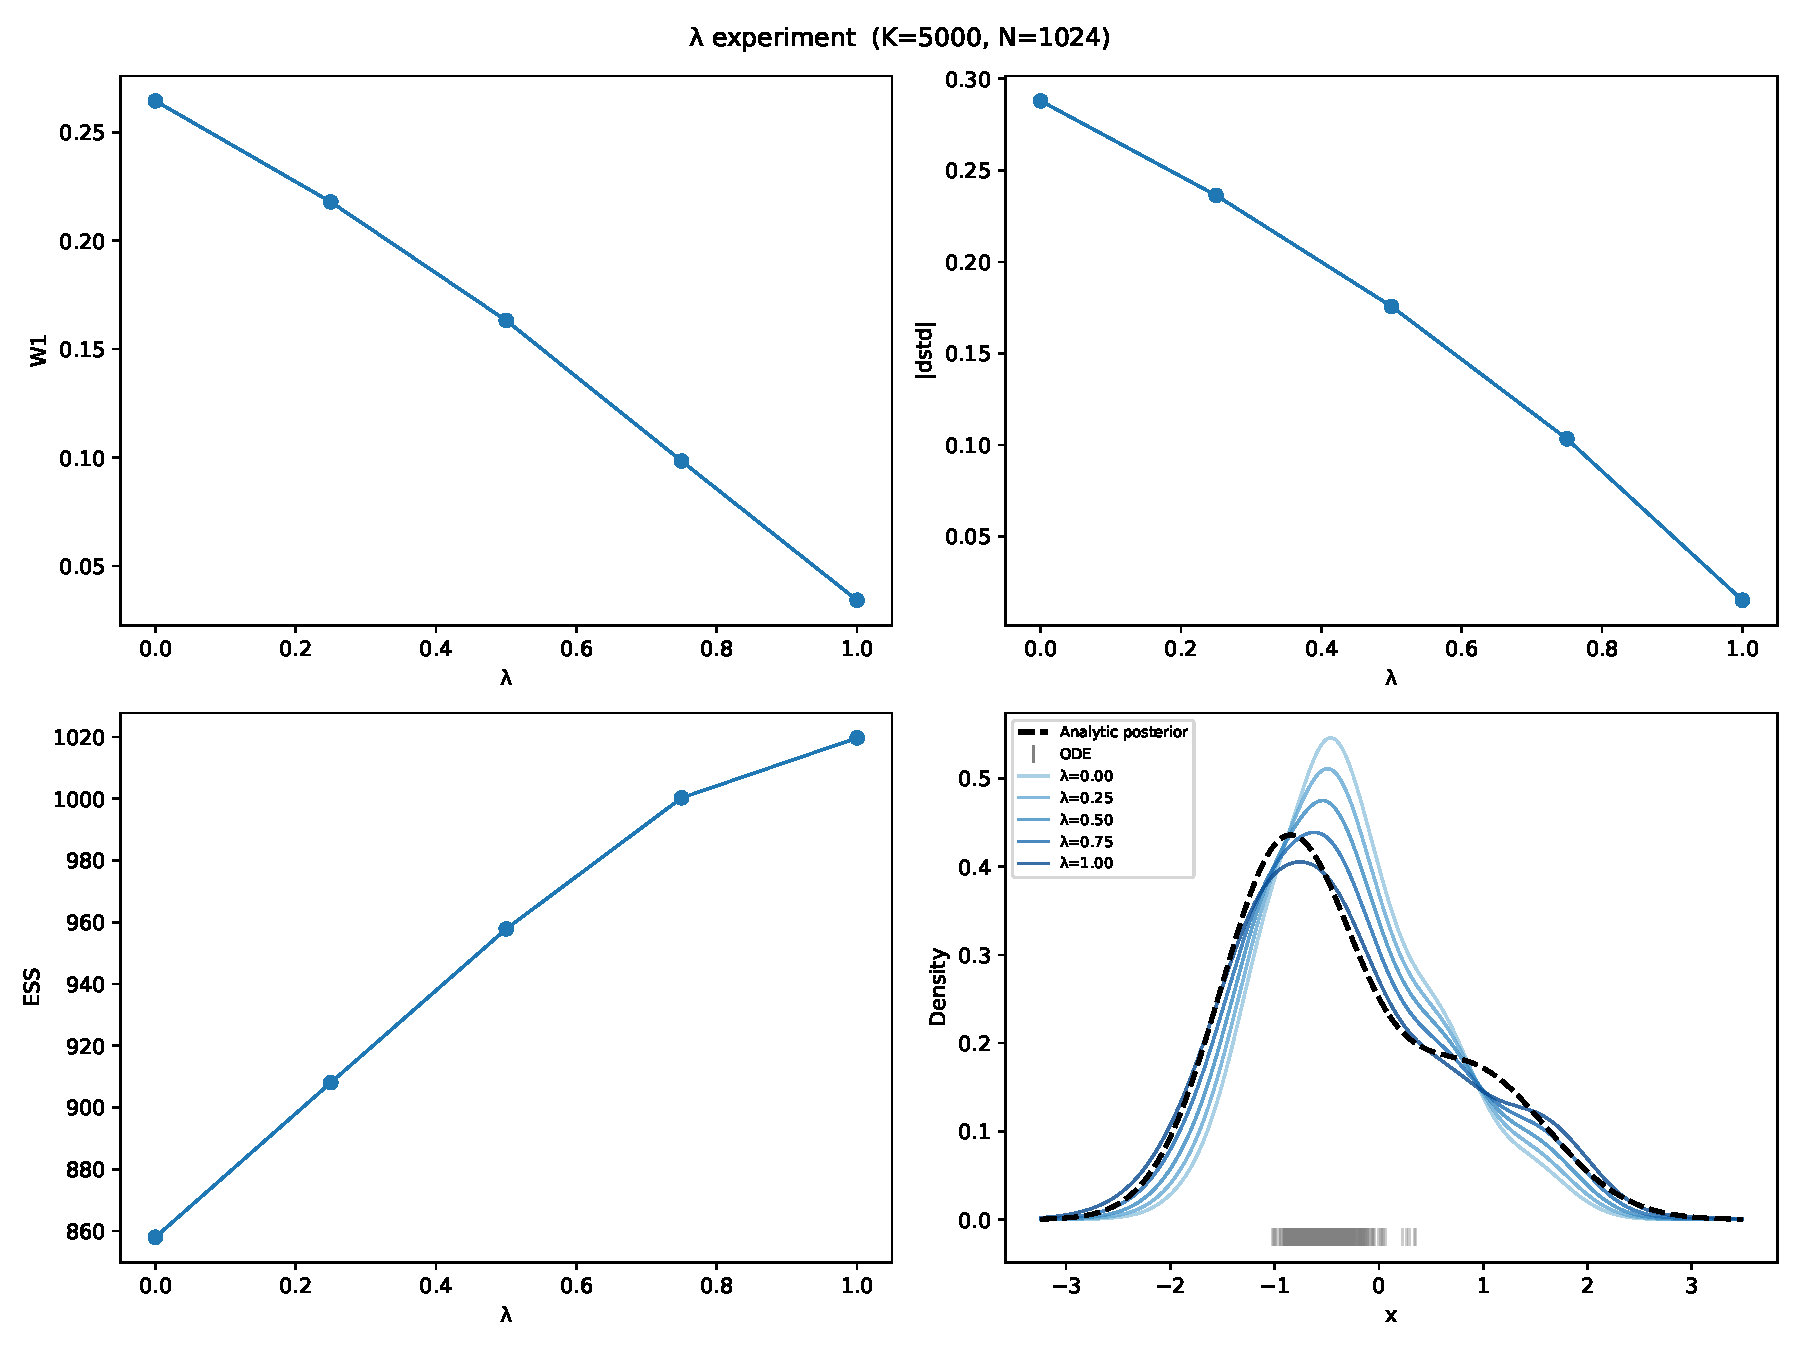
\includegraphics[width=0.85\textwidth]{figs/lambda_experiment.pdf}
\caption{$\lambda$ sweep ($K=5000$, $N=1024$).}
\label{fig:lambda}
\end{figure}

\begin{figure}[ht]
\centering
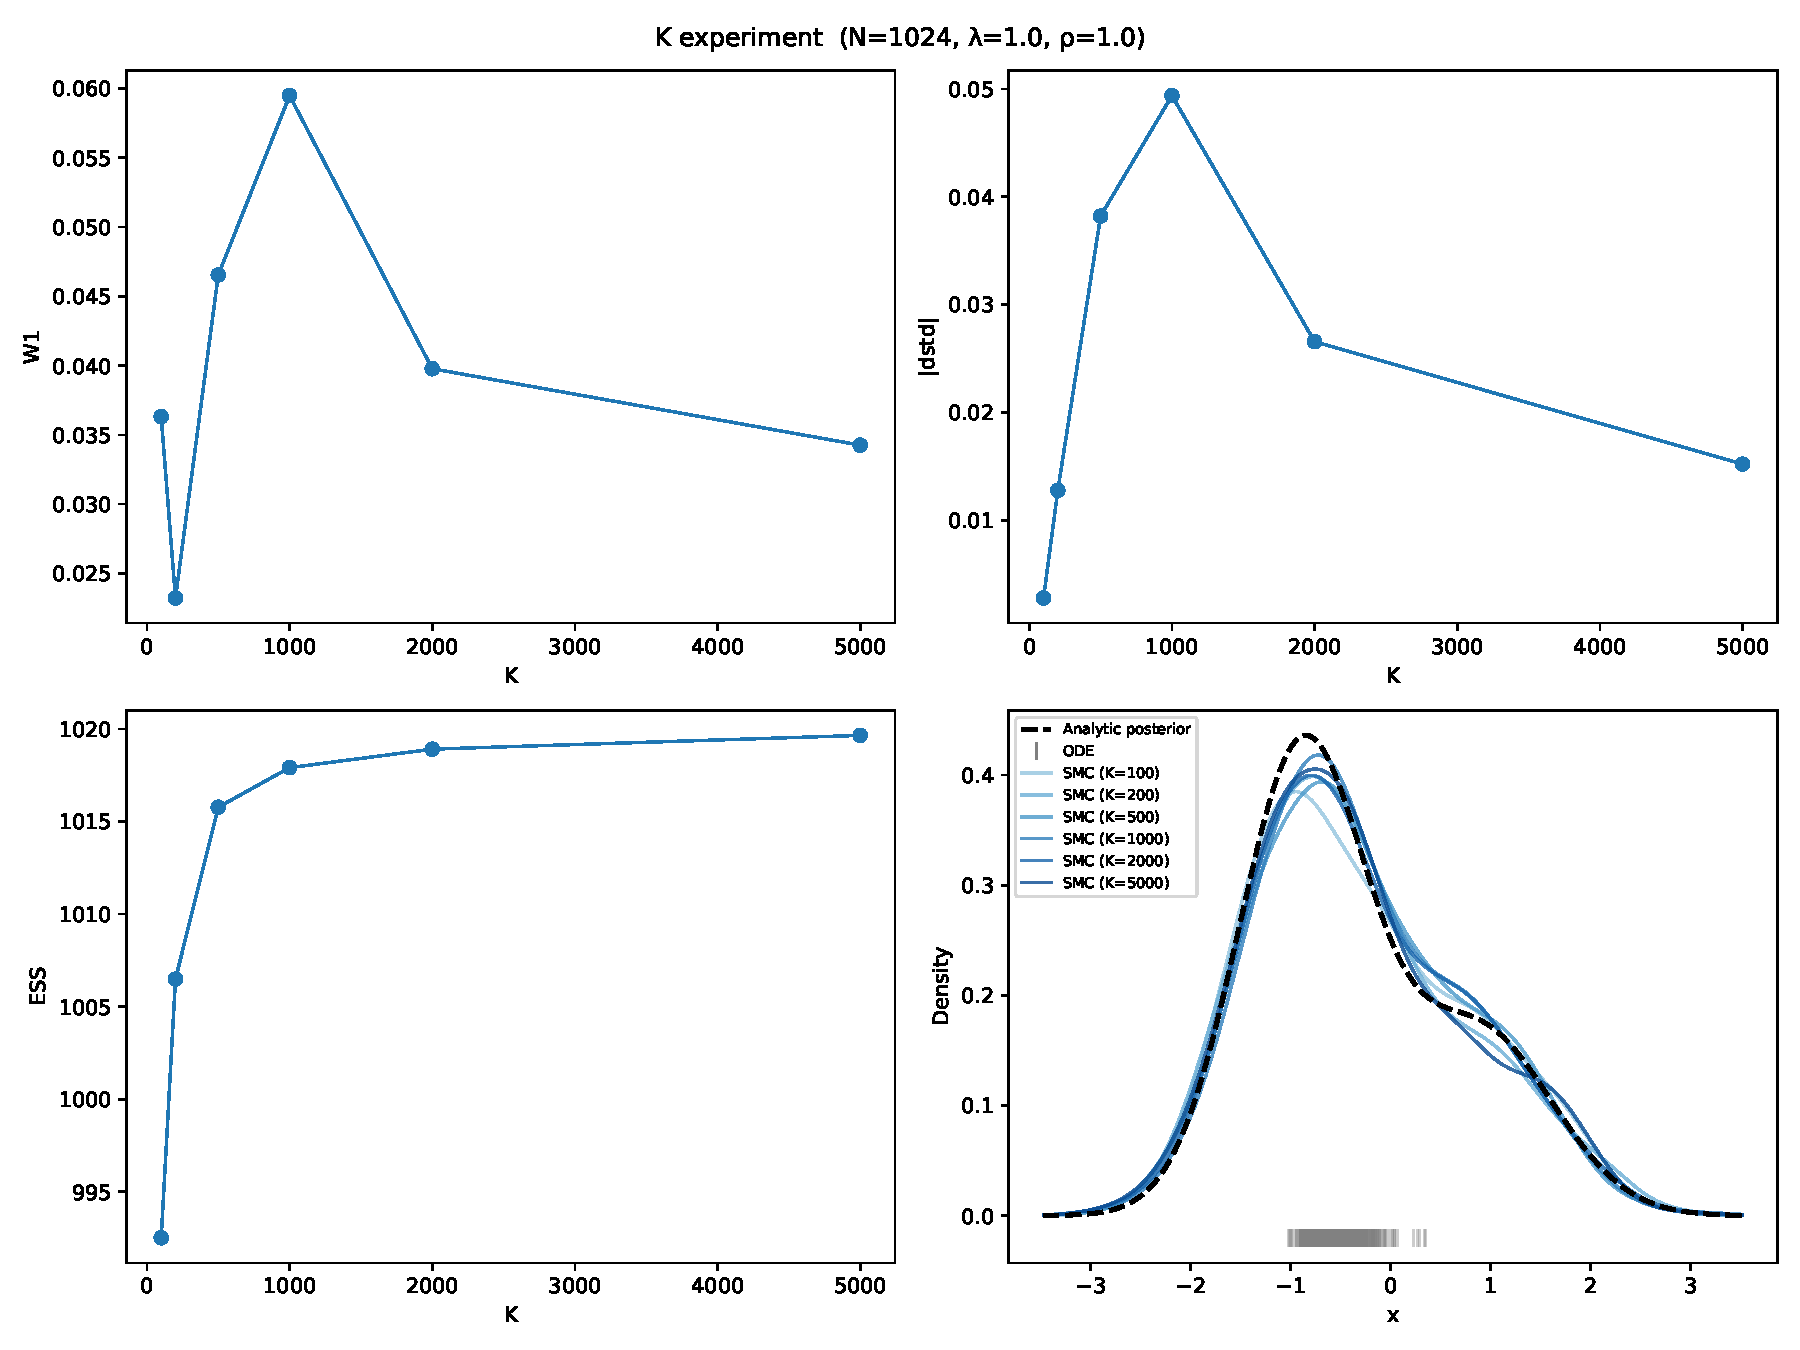
\includegraphics[width=0.85\textwidth]{figs/K_experiment.pdf}
\caption{$K$ sweep ($\lambda=1$, $N=1024$).}
\label{fig:K}
\end{figure}

\begin{figure}[ht]
\centering
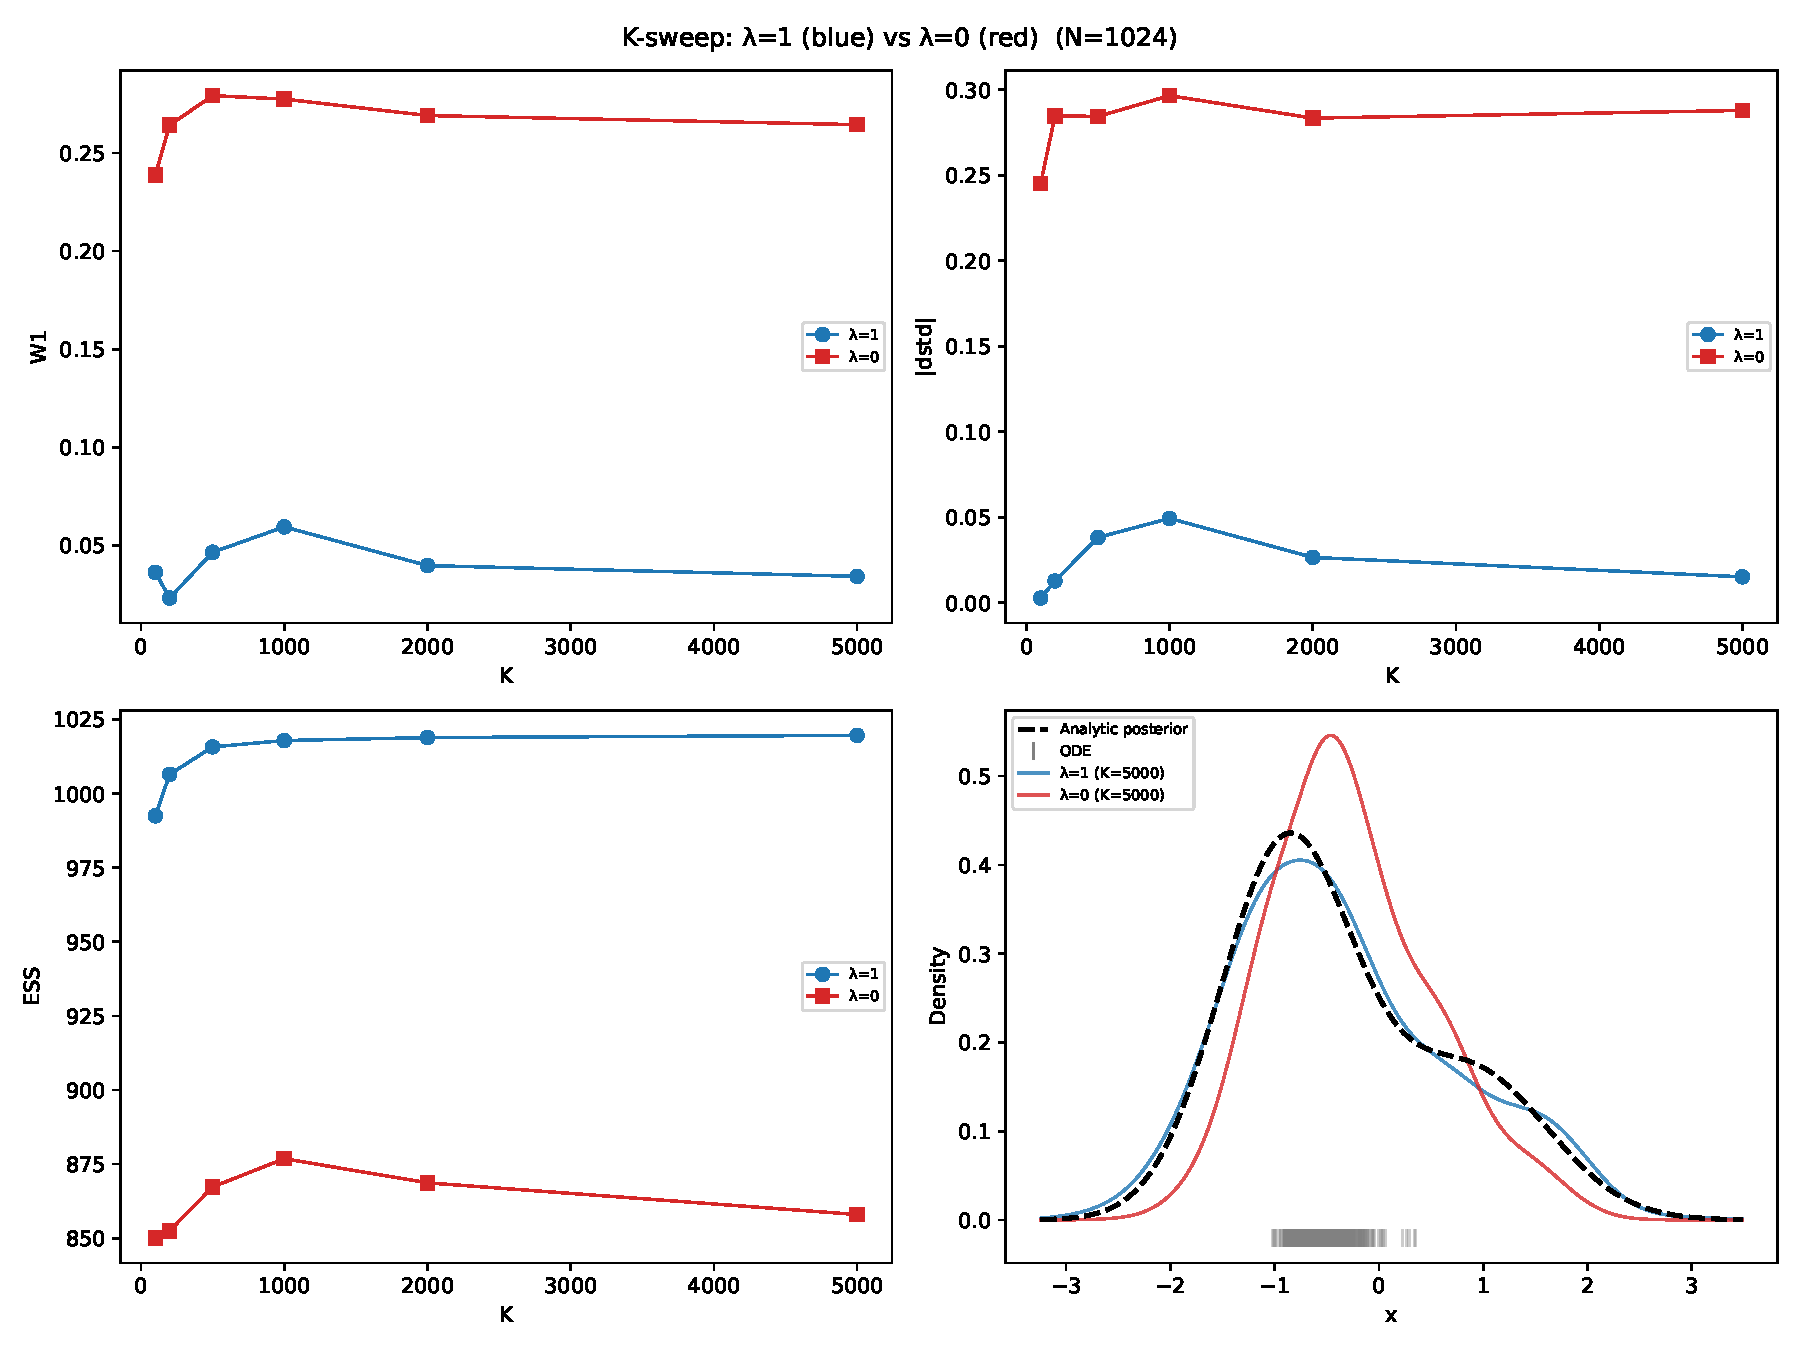
\includegraphics[width=0.85\textwidth]{figs/K_lambda_comparison.pdf}
\caption{$\lambda$ comparison $K$-sweep ($N=1024$).}
\label{fig:lambda-comp}
\end{figure}

\section{PDE-constrained reconstruction}\label{sec:pde}

The same machinery transfers to PDE-constrained reconstruction (Burgers and Darcy
solvers), where the prior is a pretrained diffusion model over solution fields and the
likelihood combines sparse sensor observations with a PDE residual.
The exact intermediate likelihood of the toy, \eqref{eq:exact-likelihood}, is intractable
in this setting; the guided samplers replace it with a surrogate formed from scaled
observation and residual losses, whose gradient plays the role of the guidance drift
\eqref{eq:guidance-drift}.
The weighting machinery of Section~\ref{sec:toy-k-sweep} transfers directly.
Details of scaling, sensor masks, and the experimental design are deferred; the toy model
above serves as the closed-form ground truth for the weighting machinery before any
trained network is involved.

\clearpage
\appendix

\section{Euler-Maruyama kernel ratio}\label{app:girsanov-euler}

For the Euler-Maruyama discretisation, both the unguided kernel
$p(x_{k-1}\mid x_k)$ and the guided proposal $q(x_{k-1}\mid x_k)$ are Gaussian
with common covariance $\delta_k I$, differing only in their means:
\begin{align*}
  p(x_{k-1}\mid x_k) &= \mathcal{N}\bigl(x_{k-1};\; \mu_p,\; \delta_k I\bigr),\\
  \mu_p &\coloneqq x_k + \delta_k\,\nabla_{x_k}\!\log p(x_k),\\[2pt]
  q(x_{k-1}\mid x_k) &= \mathcal{N}\bigl(x_{k-1};\; \mu_q,\; \delta_k I\bigr),\\
  \mu_q &\coloneqq x_k + \delta_k\bigl(\nabla_{x_k}\!\log p(x_k) + b_k\bigr)
          = \mu_p + \delta_k b_k.
\end{align*}
Drawing $x_{k-1}$ from $q$ gives $x_{k-1} = \mu_q + \sqrt{\delta_k}\,z_k$ with
$z_k \sim \mathcal{N}(0,I)$.
The log density ratio is therefore
\begin{align*}
  \log\frac{p(x_{k-1}\mid x_k)}{q(x_{k-1}\mid x_k)}
  &= -\frac{1}{2\delta_k}\Bigl(
       \|x_{k-1}-\mu_p\|^2 - \|x_{k-1}-\mu_q\|^2\Bigr)\\[2pt]
  &= -\frac{1}{2\delta_k}\Bigl(
       \|\sqrt{\delta_k}z_k + \delta_k b_k\|^2 - \|\sqrt{\delta_k}z_k\|^2\Bigr)\\[2pt]
  &= -\sqrt{\delta_k}\;b_k^\top z_k - \tfrac12\delta_k\,\|b_k\|^2
     \;=\; C_k.
\end{align*}
Thus, for the Euler-Maruyama discretisation, the Girsanov correction $C_k$
equals the exact Gaussian kernel ratio identically at every step size $\delta_k$.

\section{Alternative Girsanov discretisations}\label{app:alternatives}

The left-endpoint rule~\eqref{eq:girsanov} is the simplest It\^o-consistent
single-step discretisation of the Girsanov integral.
This appendix catalogues several refinements that, though not used in the
current experiments, remain practically testable.
The It\^o-formula discretisation (B.6) is implemented and validated
in the companion toy model of \texttt{smc/toy\_mixture.py}
(see \texttt{smc/check\_toy\_mixture.py}).

\subsection{Subdiscretised Girsanov correction}

Split step~$k$ into $m$ substeps with subincrements
$\delta_{k,1},\dots,\delta_{k,m}$ such that $\sum_{j=1}^{m}\delta_{k,j}=\delta_k$.
Draw adapted Brownian subincrements $\Delta B_{k,j}=\sqrt{\delta_{k,j}}\,z_{k,j}$
and evaluate $b$ before each subincrement is drawn.
The per-step correction becomes
\begin{equation}\label{eq:subdisc}
  C_k^{\text{sub}}
  =
  -\sum_{j=1}^{m} \sqrt{\delta_{k,j}}\; b(x_{k,j})^\top z_{k,j}
  -\frac12\sum_{j=1}^{m} \delta_{k,j}\,\|b(x_{k,j})\|^2.
\end{equation}
This is It\^o-adapted and converges to the continuous Girsanov correction as
the submesh is refined.
Cost: $m$ additional evaluations of $b$ per step.

\subsection{It\^o-Taylor correction}

Let $H_k \coloneqq \nabla^2_{x_k}\log p(y\mid x_k)$ be the Hessian of
$\log p$.
A first-order It\^o-Taylor expansion of the stochastic integral yields
\begin{equation}\label{eq:ito-taylor}
  C_k^{\text{IT}}
  =
  -\sqrt{\delta_k}\,b_k^\top z_k
  -\frac12\delta_k\Bigl[z_k^\top H_k z_k - \operatorname{tr}(H_k)\Bigr]
  -\frac12\delta_k\,\|b_k\|^2.
\end{equation}
Cost: Hessian-vector products and a trace estimate (in high dimensions,
Hutchinson-type estimation is required for $\operatorname{tr}(H_k)$).
Following the substitution of It\^o's formula to completion yields the
It\^o-formula discretisation of Appendix~\ref{app:ito-vtau},
of which~\eqref{eq:ito-taylor} is the first-order expansion.

\subsection{Corrected midpoint and trapezoidal rules}

Midpoint and trapezoidal stochastic sums approximate a Stratonovich integral.
The conversion to an It\^o integral for diffusion coefficient $g(\tau)I$ is
\[
\int g\,b\cdot dW^{\bbQ}
=
\int g\,b\circ dW^{\bbQ}
-\frac12\int g^2\,\nabla\!\cdot\! b\; d\tau,
\]
where $\nabla\!\cdot\! b = \Delta_x\log p(y\mid x)$.
A trapezoidal rule with the correction becomes
\[
C_k^{\text{trap}}
\approx
-\frac12(b_k+b_{k-1})^\top\Delta B_k
+\frac12\delta_k\,\nabla\!\cdot\! b_k
-\frac12\delta_k\,\|b_k\|^2.
\]
A simpler hybrid keeps the left-endpoint rule for the stochastic term and
applies a higher-order quadrature only to the ordinary time integral
$-\frac12\int g^2\|b\|^2 d\tau$, e.g.\ using the predictor point:
\[
C_k^{\text{hybrid}}
=
-\sqrt{\delta_k}\,b_k^\top z_k
-\frac14\delta_k\bigl(\|b_k\|^2+\|b_{\text{pred}}\|^2\bigr).
\]
This improves part of the correction while avoiding the It\^o consistency
issue in the stochastic term.

\subsection{Approximate discrete kernel ratio}

For a non-Gaussian proposal $q$, the transition is a deterministic function
$x_{k-1} = F(x_k, z_k)$.
If $F$ is invertible in $z_k$,
\[
q(x_{k-1}\mid x_k)
=
\phi(z_k)
\Bigl|\det\frac{\partial x_{k-1}}{\partial z_k}\Bigr|^{-1},
\]
where $\phi$ is the standard Gaussian density.
A corresponding evaluation for the unguided kernel $p(x_{k-1}\mid x_k)$ gives
the discrete kernel ratio directly, targeting the finite-step proposal more
accurately than a continuous-time Girsanov approximation.
Cost: inverse maps and log-determinant computations, usually prohibitive in
high dimensions; approximate log-determinants can be estimated with trace methods.

\subsection{Heuristic predictor-point correction}

Replacing $b_k$ with $b_{\text{pred}}$ in~\eqref{eq:girsanov},
\[
C_k^{\text{pred}}
=
-\sqrt{\delta_k}\,b_{\text{pred}}^\top z_k
-\tfrac12\delta_k\,\|b_{\text{pred}}\|^2,
\]
is sometimes used as an empirical heuristic.
Because $x_{\text{pred}}$ depends on the same $z_k$, this is not an
It\^o-consistent discretisation without additional correction terms.
Its performance can be tested experimentally but should not be claimed as an
automatic higher-order Girsanov rule.

\subsection{It\^o-formula discretisation}
\label{app:ito-vtau}

Applying It\^o's formula to $\ell_\tau(x)\coloneqq\log p(y\mid
x_{\sigma(\tau)}=x)$ under the guided process~\eqref{eq:sde-guided}
eliminates the stochastic integral from~\eqref{eq:step-integral} entirely.
The per-step correction becomes
\begin{align}
  C_k^{\text{V}}
  &\coloneqq \int_{\tau_k}^{\tau_{k-1}} V_\tau(x_k)\,d\tau,
  \label{eq:Vtau-step}\\[2pt]
  V_\tau(x) &\coloneqq \partial_\tau\ell_\tau(x)
              + a(x,\tau)\!\cdot\!\nabla\ell_\tau(x)
              + \tfrac12\,\nabla\ell_\tau^\top\Sigma\,\nabla\ell_\tau
              + \tfrac12\operatorname{tr}\bigl(\Sigma\,\nabla^2\ell_\tau(x)\bigr),
  \label{eq:Vtau-def}
\end{align}
where the pre-step state $x_k$ is frozen during the deterministic quadrature.
The $\partial_\tau\ell_\tau$ term integrates exactly (telescoping):
$\int_{\tau_k}^{\tau_{k-1}}\partial_\tau\ell_\tau\,d\tau = \ell_{\tau_{k-1}}(x_k) - \ell_{\tau_k}(x_k)$.
In practice only the remaining part,
\begin{equation}
  H_\tau(x) \coloneqq a(x,\tau)\!\cdot\!\nabla\ell_\tau(x)
                    + \tfrac12\,\nabla\ell_\tau^\top\Sigma\,\nabla\ell_\tau
                    + \tfrac12\operatorname{tr}\bigl(\Sigma\,\nabla^2\ell_\tau(x)\bigr),
  \label{eq:Htau-def}
\end{equation}
requires numerical quadrature, giving
$C_k^{\text{V}} = \ell_{\tau_{k-1}}(x_k) - \ell_{\tau_k}(x_k) + \int_{\tau_k}^{\tau_{k-1}} H_\tau(x_k)\,d\tau$
(\texttt{smc/check\_toy\_mixture.py}).

In the variance-exploding parametrisation ($\Sigma=\bar a I$,
$a(x,\tau)=\bar a\,\nabla\!\log p$, $\partial_\tau=-\partial_\sigma$,
$\bar a(\tau)\coloneqq 2\sigma(\tau)$) this reduces to
$H_\tau = \bar a\,\nabla\!\log p\!\cdot\!\nabla\ell
        + \tfrac12\bar a\,\|\nabla\ell\|^2
        + \tfrac12\bar a\,\Delta\ell$.

Unlike the left-endpoint rule~\eqref{eq:girsanov} and its
variants~\eqref{eq:subdisc}--\eqref{eq:ito-taylor},
\eqref{eq:Vtau-step} contains \emph{no stochastic term} --- the per-step
weight is a deterministic function of $x_k$.
The price is the Laplacian $\Delta\ell=\operatorname{tr}(\nabla^2\ell)$,
which in high dimensions requires stochastic estimation
(cf.\ Hutchinson-type trace estimators; \texttt{smc/hutchinson.py}).
In one dimension $\Delta\ell$ reduces to an exact second derivative via
double backward differentiation.
The It\^o-Taylor correction~\eqref{eq:ito-taylor} is the first-order
expansion of~\eqref{eq:Vtau-step} that \emph{retains} the stochastic term
while adding a Hessian-based correction;
$C_k^{\text{V}}$ completes the substitution by eliminating it entirely.

\bibliographystyle{plainnat}
\bibliography{references_2}

\end{document}
